\documentclass[master=ene]{kulemt}
\setup{title={Beste masterproef ooit al geschreven},
  author={},
  promotor={Prof.\,dr.\,ir.\ L. Helsen},
  assessor={Ir.\,W. Eetveel\and W. Eetrest},
  assistant={Dr.\,ir.\ M. Sourbron \and Ir.\,B.~van der Heijde}}
% De volgende \setup mag verwijderd worden als geen fiche gewenst is.
\setup{filingcard,
  translatedtitle={The best master thesis ever},
  udc=621.3,
  shortabstract={Hier komt een heel bondig abstract van hooguit 500
    woorden. \LaTeX\ commando's mogen hier gebruikt worden. Blanco lijnen
    (of het commando \texttt{\string\pa r}) zijn wel niet toegelaten!
    \endgraf \lipsum[2]}}
% Verwijder de "%" op de volgende lijn als je de kaft wil afdrukken
%\setup{coverpageonly}
% Verwijder de "%" op de volgende lijn als je enkel de eerste pagina's wil
% afdrukken en de rest bv. via Word aanmaken.
%\setup{frontpagesonly}

% Kies de fonts voor de gewone tekst, bv. Latin Modern
\setup{font=lm}

% Hier kun je dan nog andere pakketten laden of eigen definities voorzien

% Tenslotte wordt hyperref gebruikt voor pdf bestanden.
% Dit mag verwijderd worden voor de af te drukken versie.
\usepackage[pdfusetitle,colorlinks,plainpages=false]{hyperref}

%%%%%%%
% Om wat tekst te genereren wordt hier het lipsum pakket gebruikt.
% Bij een echte masterproef heb je dit natuurlijk nooit nodig!
\IfFileExists{lipsum.sty}%
 {\usepackage{lipsum}\setlipsumdefault{11-13}}%
 {\newcommand{\lipsum}[1][11-13]{\par Hier komt wat tekst: lipsum ##1.\par}}
%%%%%%%

%\includeonly{hfdst-n}
\begin{document}

\begin{preface}
  Dit is mijn dankwoord om iedereen te danken die mij bezig gehouden heeft.
  Hierbij dank ik mijn promotor, mijn begeleider en de voltallige jury.
  Ook mijn familie heeft mij erg gesteund natuurlijk.
\end{preface}

\tableofcontents*

\begin{abstract}
  In dit \texttt{abstract} environment wordt een al dan niet uitgebreide
  samenvatting van het werk gegeven. De bedoeling is wel dat dit tot
  1~bladzijde beperkt blijft.

  \lipsum[1]
\end{abstract}

% Een lijst van figuren en tabellen is optioneel
%\listoffigures
%\listoftables
% Bij een beperkt aantal figuren en tabellen gebruik je liever het volgende:
\listoffiguresandtables
% De lijst van symbolen is eveneens optioneel.
% Deze lijst moet wel manueel aangemaakt worden, bv. als volgt:
\chapter{Lijst van afkortingen en symbolen}
\section*{Afkortingen}
\begin{flushleft}
  \renewcommand{\arraystretch}{1.1}
  \begin{tabularx}{\textwidth}{@{}p{12mm}X@{}}
    LoG   & Laplacian-of-Gaussian \\
    MSE   & Mean Square error \\
    PSNR  & Peak Signal-to-Noise ratio \\
  \end{tabularx}
\end{flushleft}
\section*{Symbolen}
\begin{flushleft}
  \renewcommand{\arraystretch}{1.1}
  \begin{tabularx}{\textwidth}{@{}p{12mm}X@{}}
    42    & ``The Answer to the Ultimate Question of Life, the Universe,
            and Everything'' volgens de \cite{h2g2} \\
    $c$   & Lichtsnelheid \\
    $E$   & Energie \\
    $m$   & Massa \\
    $\pi$ & Het getal pi \\
  \end{tabularx}
\end{flushleft}

% Nu begint de eigenlijke tekst
\mainmatter

\chapter{Inleiding}
\label{inleiding}
In dit hoofdstuk wordt het werk ingeleid. Het doel wordt gedefinieerd en er
wordt uitgelegd wat de te volgen weg is (beter bekend als de rode draad).

Als je niet goed weet wat een masterproef is, kan je altijd
Wikipedia\cite{wiki} eens nakijken.

\section{Lorem ipsum 4--5}
\lipsum[4-5]

\section{Lorem ipsum 6--7}
\lipsum[6-7]

%%% Local Variables: 
%%% mode: latex
%%% TeX-master: "masterproef"
%%% End: 

\chapter{Het eerste hoofdstuk}
\label{hoofdstuk:1}
Een hoofdstuk behandelt een samenhangend geheel dat min of meer op zichzelf
staat. Het is dan ook logisch dat het begint met een inleiding, namelijk
het gedeelte van de tekst dat je nu aan het lezen bent.

\section{Eerste onderwerp in dit hoofdstuk}
De inleidende informatie van dit onderwerp.

\subsection{Een item}
De bijbehorende tekst. Denk eraan om de paragrafen lang genoeg te maken en
de zinnen niet te lang.

Een paragraaf omvat een gedachtengang en bevat dus steeds een paar zinnen.
Een paragraaf die maar \'e\'en lijn lang is, is dus uit den boze.

\section{Tweede onderwerp in dit hoofdstuk}
Er zijn in een hoofdstuk verschillende onderwerpen. We zullen nu
veronderstellen dat dit het laatste onderwerp is.

\subsection{Een item}
Maak ook geen misbruik van opsommingen. Voor korte opsommingen gebruik je
geen ``\verb|itemize|'' of ``\texttt{enumerate}'' commando's. Doe dus
\emph{niet} het volgende:
\begin{quote}
  De Eiffeltoren bevat drie verdiepingen:
  \begin{itemize}
  \item de eerste;
  \item de tweede;
  \item de derde.
  \end{itemize}
\end{quote}
Maar doe:
\begin{quote}
  De Eiffeltoren bevat drie verdiepingen: de eerste, de tweede en de derde.
\end{quote}

\section{Besluit van dit hoofdstuk}
Als je in dit hoofdstuk tot belangrijke resultaten of besluiten gekomen
bent, dan is het ook logisch om het hoofdstuk af te ronden met een
overzicht ervan. Voor hoofdstukken zoals de inleiding en het
literatuuroverzicht is dit niet strikt nodig.

%%% Local Variables: 
%%% mode: latex
%%% TeX-master: "masterproef"
%%% End: 

\documentclass[a4paper,oneside,11pt]{report}

% Packages laden
\usepackage[a4paper,top=2cm,bottom=2cm,left=3cm,right=2cm]{geometry}		% paginagrootte
\usepackage{parskip}					% andere regels voor nieuwe paragraaf: witregel + niet inspringen

\usepackage[latin1]{inputenc}					% invoer van speciale tekens (bvb. Umlaut)
\usepackage{lmodern}						% betere weergave van speciale tekens (bvb. Umlaut)
\usepackage{dsfont}	
\usepackage{amsfonts,amsthm, tabularx}			% wiskundige symbolen and table of equations
%\usepackage{mathtools}
\usepackage{enumerate}

\usepackage{graphicx,subcaption}					% figuren
\usepackage{float}								% plaatsen van figuren en tabellen
\usepackage[font=small,labelfont=bf]{caption}
\usepackage[format=plain,indent=1cm]{caption}
\usepackage{eurosym}
\usepackage[squaren,Gray]{SIunits}
\usepackage{amsmath,amsfonts,amsthm,mathrsfs,MnSymbol}	% wiskundige symbolen
\usepackage{pifont}	
\usepackage{color}				% Load the color package: \color{declared-color}{text}. If also background:
								% \colorbox{declared-color1}{\color{declared-color2}text}
\usepackage[dutch]{babel}		% spellingcorrectie Nederlands
\usepackage{titling}
\usepackage{epstopdf}
\usepackage{stackengine}
\usepackage{graphicx}
\usepackage{hyperref}

\graphicspath{{./Figures/}}
	% personaliseren van onderschriften
\captionsetup[table]{name=Tabel}
							% sign of euro


% Instellingen voor document
\renewcommand{\arraystretch}{1.1}				% tabelrijen iets hoger maken
\urlstyle{same}
\hypersetup{hidelinks=true}

\renewcommand*\thesection{\arabic{section}}
\DeclareMathOperator*{\argmin}{\arg\!\min}

\numberwithin{figure}{section}
\numberwithin{table}{section}
\numberwithin{equation}{section}					

\setcounter{secnumdepth}{3}		% Enable subsubsection numbering
\setcounter{tocdepth}{3}		% Include subsubsection in table of content

\pagenumbering{arabic}

\begin{document}
%\pagenumbering{gobble}
\newpage


\section{Definitie}

De meest algemene definitie van de ladingstoestand (SoC) is de verhouding tussen de huidige energie-inhoud $E(t)$ en de maximale energie-inhoud $E_{max}$ die een boorveld kan bezitten. \cite{R28}
\\ \begin{equation}\label{def_eq1}
SoC=\dfrac{E(t)}{E_{max}}
\end{equation}

In de diepte bestaat een boorveld uit verschillende lagen aangezien de bodemeigenschappen van de verschillende bodemlagen sterk kunnen verschillen. Stel nu dat het boorveld bestaat uit N lagen, dan kan voor elke laag n de ladingstoestand, $SoC_n$ opgesteld worden. De totale ladingstoestand, $SoC_{tot}$, volgt dan uit deze individuele ladingstoestanden. Figuur \ref{fig:def_1} toont de doorsnede van een U-boorveld met 2 lagen. 

\begin{figure}[hbtp] 
	\centering
	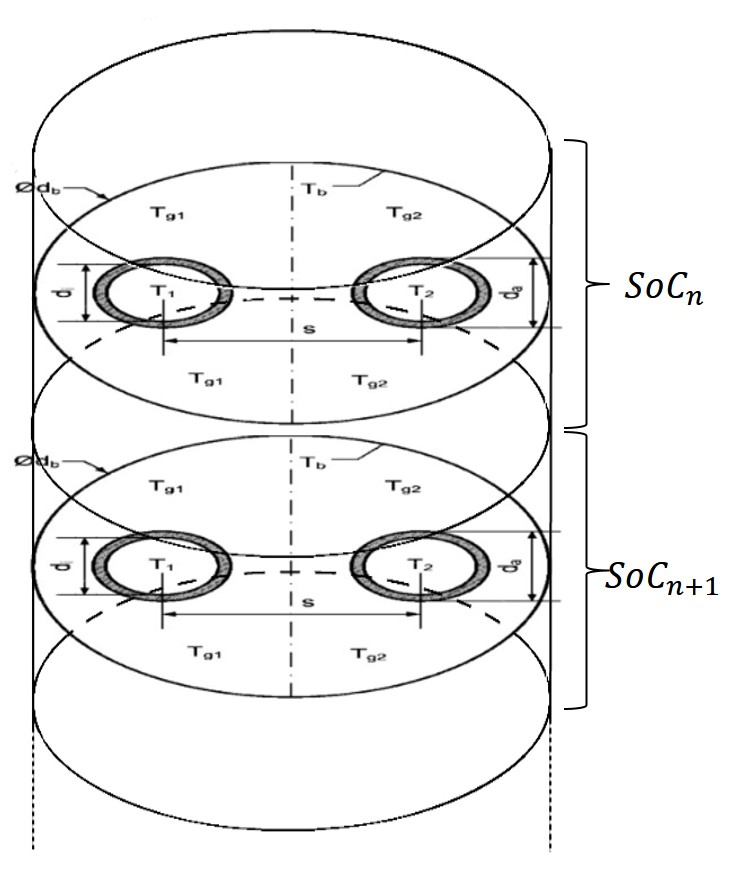
\includegraphics[width=0.4 \textwidth]{def_fig1.jpg}
	\caption{Doorsnede van een U-boorveld met 2 lagen.}
	\label{fig:def_1}
\end{figure}
 

Door gebruik te maken van thermische weerstanden en thermische warmtecapaciteiten, kan per laag een equivalent schema opgesteld worden, zoals getoond in Figuur \ref{fig:def_2} en Figuur \ref{fig:def_3} \cite{R23}. Met behulp van dit equivalent schema is de definitie voor de ladingstoestand van laag n, $SoC_n$,  de volgende.\cite{R28}\\
\begin{equation}\label{def_eq2}
SoC_n=\dfrac{\sum\limits_{i=1}^k m_{i,n}.c_{p_{i,n}}.(T_{i,n}(t)-T_{n,ref})}{\sum\limits_{i=1}^k m_{i,n}.c_{p_{i,n}}.(T_{i,n,max}-T_{n,ref})}
\end{equation}
Hieruit volgt dan ook de definitie van de totale ladingstoestand, $SoC_{tot}$ door te sommeren over de verschillende lagen.
\\
\begin{equation}\label{def_eq3}
SoC_{tot}=\dfrac{\sum\limits_{n=1}^N \sum\limits_{i=1}^k m_{i,n}.c_{p_{i,n}}.(T_{i,n}(t)-T_{n,ref}) }{\sum\limits_{n=1}^N \sum\limits_{i=1}^k m_{i,n}.c_{p_{i,n}}.(T_{i,n,max}-T_{n,ref})}
\end{equation}

\begin{figure}[hbtp] 
	\centering
	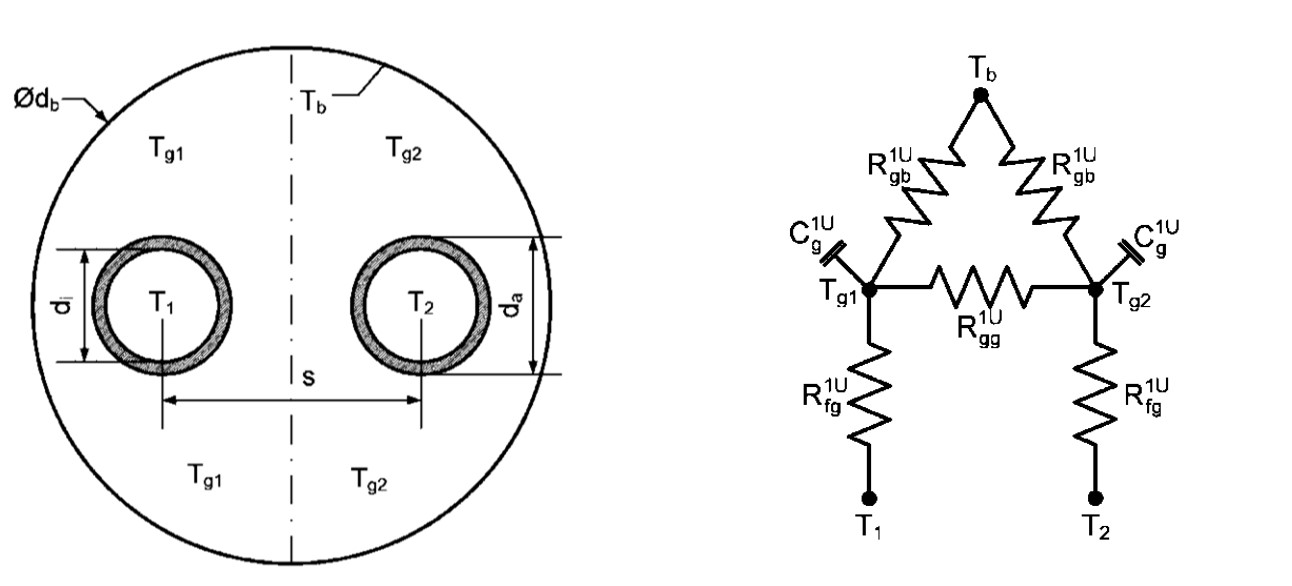
\includegraphics[width=0.8 \textwidth]{def_fig2.jpg}
	\caption{Equivalent schema van \'e\'en laag.}
	\label{fig:def_2}
\end{figure}

\begin{figure}[hbtp] 
	\centering
	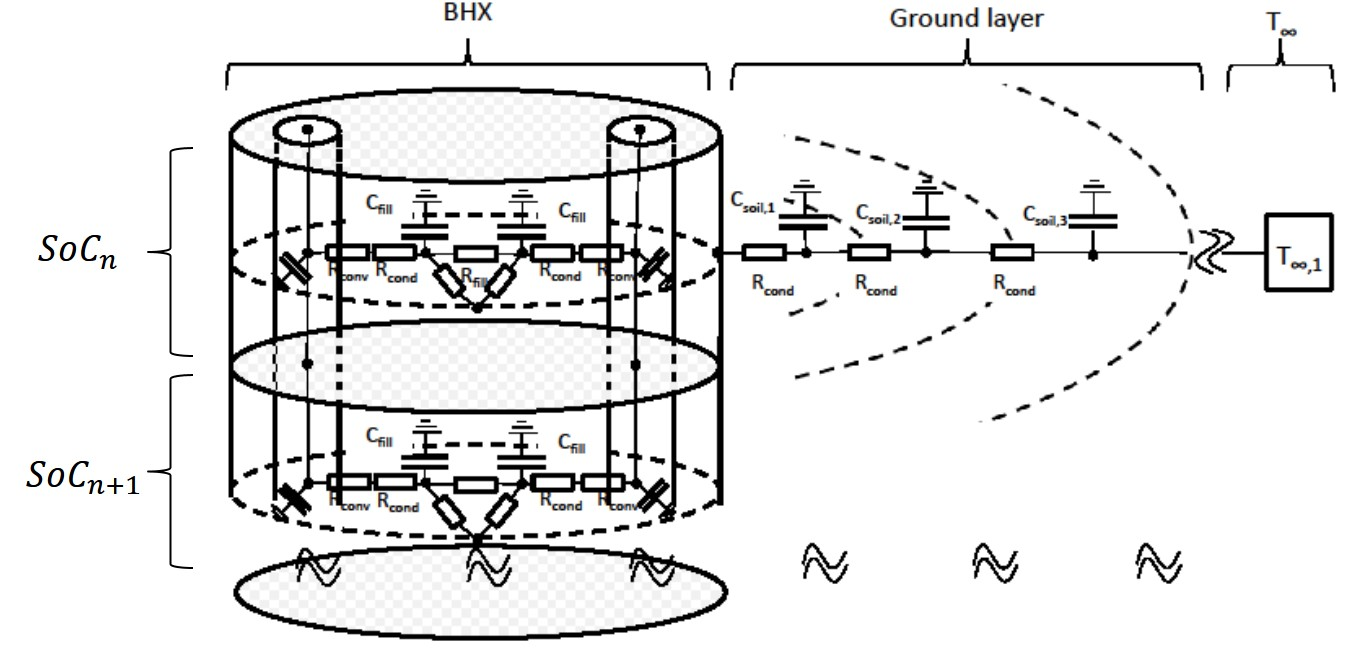
\includegraphics[width=0.8 \textwidth]{def_fig3.jpg}
	\caption{Weergave van het equivalent schema voor verschillende lagen.}
	\label{fig:def_3}
\end{figure}


\textcolor{red}{In Modelica bibliotheek "IDEAS" is er een model beschikbaar dat zowel korte termijn als lange termijn combineert (Damien Picard en Prof. Helsen) \cite{R7}, \cite{R25}.} 
  


Een belangrijke input in dit model is de referentietemperatuur. Een eerste mogelijke keuze is het gebruiken van de wettelijke temperatuurslimiet. Deze wettelijke limiet ligt in Belgi\"e op een minimum van 0 \degree C en een maximum van 25 \degree C \cite{}. Bij deze keuze behaalt de ladingstoestand waarschijnlijk nooit een waarde van 0 of 1 aangezien de temperatuur deze limieten niet bereikt. 
Een tweede optie bestaat erin om de technische limieten te gebruiken. Bijvoorbeeld voor koeling van een gebouw moet de grondtemperatuur lager blijven dan de temperatuur die nodig is om de ruimte te koelen. Maar tegelijkertijd moet de grondtemperatuur ook hoger zijn dan de vriestemperatuur van het koelmiddel. 
\begin{equation} \label{def_eq4}
T_{vries}<T_{grond}<T_{aanvoer,koeling}
\end{equation}
Analoog voor de verwarming van een gebouw.
\begin{equation}\label{def_eq5}
T_{aanvoer,verwarming}<T_{grond}<T_{kook}
\end{equation}
Om de grootste range, van waarde 0 tot 1, van de ladingstoestand te behalen is het nuttig om de werkelijke gebruikslimieten te gebruiken. Deze werkelijke gebruikslimieten kunnen veranderlijk zijn in de tijd. 

\newpage
\section{Invloedsfactoren}
Om een gepast model op te stellen, is het belangrijk de invloed van parameters en eigenschappen te kennen en welke nauwelijks invloed hebben. Belangrijk hierbij op de merken is dat de bepaling van deze parameters en eigenschappen mogelijk moet zijn, ofwel enerzijds door metingen uit te voeren of door databanken te raadplegen. 
\textcolor{red}{De gegevens moeten ook bruikbaar zijn in een regelaar.}
\par Een opsomming van de mogelijke invloedsfactoren op de ladingstoestand staat hieronder. De factoren met de grootste invloed op de ladingstoestand, onderstreept in onderstaande lijst, worden verder toegelicht. 
\begin{itemize}
\item Bodemeigenschappen
	\begin{itemize}
	\item Bodemstructuur en materiaal van de bodem
   	\item \underline{Thermische conductiviteit} ($k$)
	\item \underline{Thermische diffusiviteit} ($\alpha$)
	\item \underline{Volumetrische warmtecapaciteit} ($c$)
	\item Porositeit ($\varphi$)
	\end{itemize}	
\item Temperatuur
	\begin{itemize}
	\item \underline{Temperatuur aan grondoppervlak}
	\end{itemize}
\item \underline{Grondwaterstroming}
\item Dimensies
	\begin{itemize}
	\item Lengte van het boorgat
	\item \underline{Lay-out van het boorgatenergieopslagveld}
	\end{itemize}
\item \underline{Bodemsaturatie}
\end{itemize}
	

\subsection*{Thermische conductiviteit, diffusiviteit en warmtecapaciteit}
De thermische conductiviteit $k$, thermische diffusiviteit $\alpha$ en de volumetrische warmtecapaciteit $c$ zijn gelinkt via volgende relatie.
\begin{equation}\label{invlf_eq1}
\alpha=\dfrac{k}{\rho.c_p}=\dfrac{k}{c}
\end{equation}
De meest geschikte toepassing van het energieopslagveld is afhankelijk van de thermische conductiviteit. Bij een grote thermische conductiviteit, regenereert de bodem snel. De bodem is dan het meest geschikt als een dissipator van energie. Dit is zo als de warmtevraag ongebalanceerd is, enkel een warmtevraag of koudevraag gedurende het hele jaar. Is de thermische conductiviteit klein, dan is de bodem geschikt als energieopslag. De warmtevraag dient dan gebalanceerd te zijn. Gedurende het jaar is er vraag naar warmte en koeling.
\par Smart Geotherm stelt geschiktheidskaarten ter beschikking. Er zijn kaarten verkrijgbaar voor de gemiddelde thermische conductiviteit (Figuur \ref{fig:invlf_1}), de maximale gemiddelde thermische conductiviteit (Figuur \ref{fig:invlf_2}) en de minimale gemiddelde thermische conductiviteit (Figuur \ref{fig:invlf_3}) voor een diepte van 100 m of tot de diepte van een vaste rots \cite{}. De gemiddelde thermische conductiviteit bepaalt meestal de meest geschikte toepassing. Sectie \ref{}  behandelt de invloed van het gebruik van de gemiddelde, maximale of minimale thermische conductiviteit op de ladingstoestand. 

\textcolor{red}{Tekst toevoegen: Vereenvoudiging lagen door equivalente parameters.}

\begin{figure}[hbtp] 
	\centering
	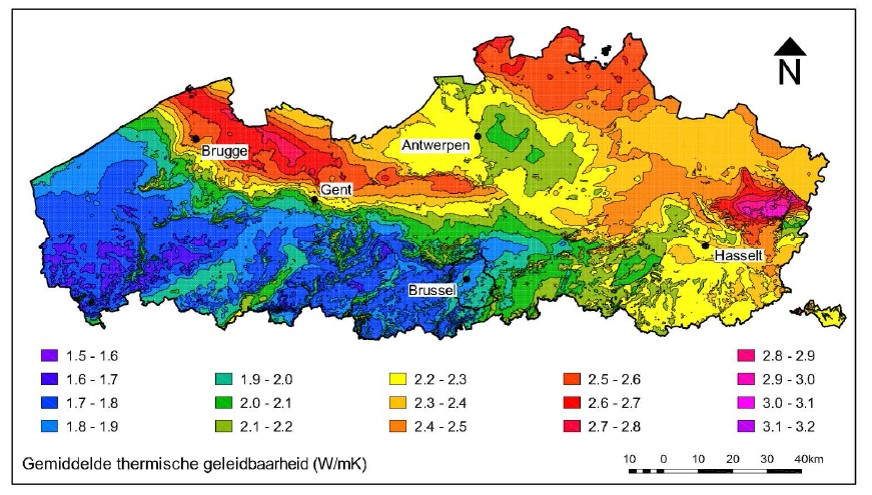
\includegraphics[width=0.7 \textwidth]{invlf_fig1.jpg}
	\caption{Gemiddelde thermische geleidbaarheid tot op een diepte van 100 m of tot op de vaste rots.}
	\label{fig:invlf_1}
\end{figure}

\begin{figure}[hbtp] 
	\centering
	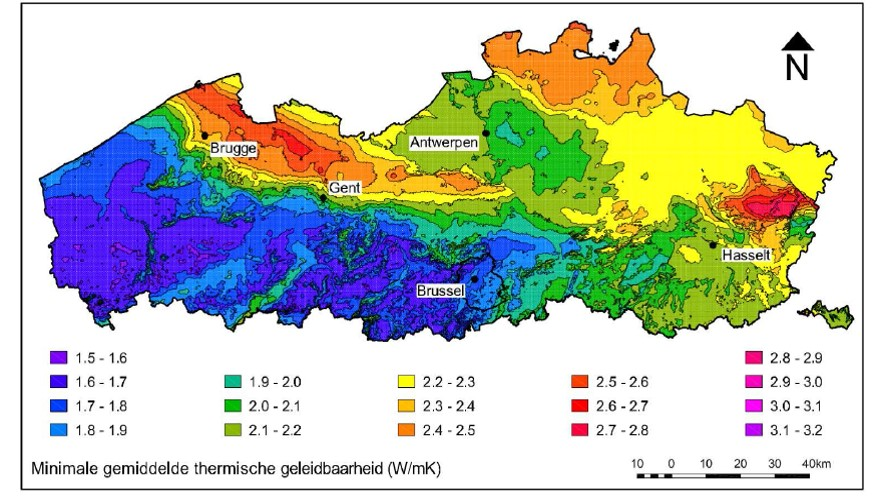
\includegraphics[width=0.7 \textwidth]{invlf_fig2.jpg}
	\caption{Minimale gemiddelde thermische geleidbaarheid tot op een diepte van 100 m of tot op de vaste rots.}
	\label{fig:invlf_2}
\end{figure}

\begin{figure}[hbtp] 
	\centering
	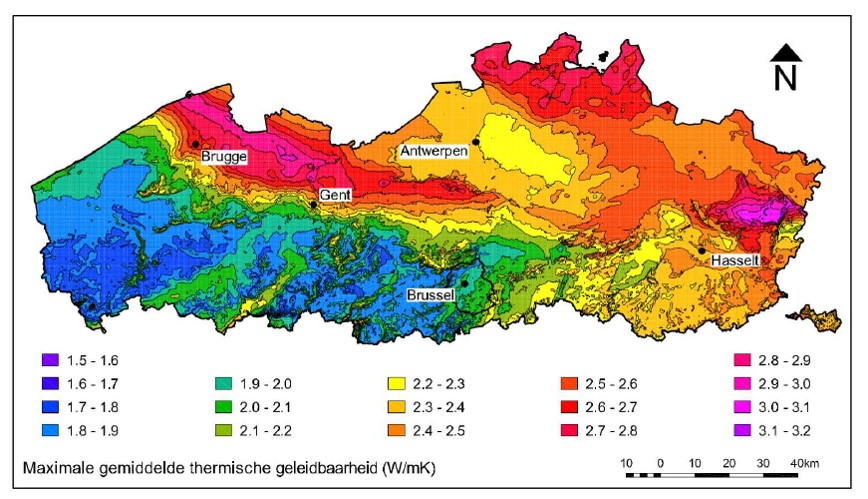
\includegraphics[width=0.7 \textwidth]{invlf_fig3.jpg}
	\caption{Maximale gemiddelde thermische geleidbaarheid tot op een diepte van 100 m of tot op de vaste rots.}
	\label{fig:invlf_3}
\end{figure}


\subsection*{Temperatuur van grondoppervlak}
Vooral de bovenste lagen van de bodem ondervinden een invloed van de buitentemperatuur aan het grondoppervlak. Figuur \ref{fig:invlf_4} geeft dit temperatuursverloop weer. Vanaf een diepte van 10 \'a 30 m is de temperatuur nagenoeg constant (10 - 12 \degree C). Hierna stijgt de temperatuur met 3 \degree C per 100 m \cite{}. Indien deze eerste 10 \'a 30 m relatief een significant deel vormt van de diepte van het boorgat, dient dit temperatuursverloop in rekening gebracht te worden. 
 
\begin{figure}[hbtp] 
	\centering
	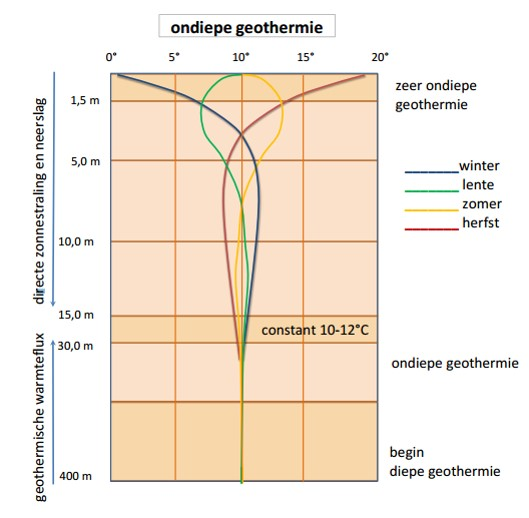
\includegraphics[width=0.45 \textwidth]{invlf_fig4.jpg}
	\caption{Temperatuursverloop in functie van de diepte.}
	\label{fig:invlf_4}
\end{figure}

\subsection*{Grondwaterstroming}
De eventuele aanwezigheid van grondwaterstroming heeft een invloed op de temperatuurverdeling rondom het boorveld. Indien de temperatuurverdeling niet meer symmetrisch is rondom het boorgatenergieopslagveld heeft dit een invloed op de modellering. Grondwaterstroming zorgt ervoor dat de bodem sneller regenereert waardoor het geschikt is voor energiedissipatie.
Een karakteristiek getal voor grondwaterstroming is het P\'eclet-getal \cite{}. 
\begin{equation} \label{invlf_eq2}
Pe=\dfrac{r_b.v}{\alpha}=\dfrac{r_b.\Phi}{\alpha.\varphi}
\end{equation}
Hierbij is $v$ niet de snelheid waarmee de vloeistof door de pori\"en stroomt, maar wel de Darcysnelheid. Slechts een fractie van het volume is echter beschikbaar voor stroming. 

\subsection*{Lay-out}
De lay-out van een boorveld kan een lijn of een meer compacte vorm, een matrix vorm, zijn. (Figuur 7) Samen met de eventuele aanwezigheid van grondwaterstroming heeft de lay-out een sterke invloed op de temperatuurverdeling, op het temperatuursverloop in de tijd, alsook de tijd om een evenwichtstoestand te bereiken en op de effici\"entie van het boorgatenergieopslagveld. Ook het feit of de vraag gebalanceerd of ongebalanceerd is speelt een rol.
\par Bij volgende simulaties werd de invloed van de temperatuur van het grondoppervlak verwaarloosd \cite{R10}. Voor een gebalanceerde vraag met grondwaterstroming heeft grondwaterstroming nauwelijks effect, ongeacht de lay-out. Indien de vraag daarentegen ongebalanceerd is, kan dit een sterke invloed hebben op het temperatuursverloop \cite{R10}. (Figuur 8)
\par Bij een ongebalanceerde vraag is de invloed van grondwaterstroming significant. Het koudste punt van de temperatuurverdeling verplaatst zich stroomafwaarts buiten het middelpunt van de matrix lay-out. Figuur \ref{fig:invlf_7} geeft de temperatuurverdeling van een boorgatenergieopslagveld met matrix lay-out weer\cite{R10}. 
\par De invloed van de lay-out bij een ongebalanceerde warmtevraag en zonder grondwaterstroming is weergegeven in Figuur \ref{fig_invlf_8}. Hierbij dient aandacht besteed te worden aan de afstandsschaal. 10 m buiten het middelpunt bij de matrix lay-out bereikt de grond gemiddeld een temperatuur van 4 \degree C. Bij de lijn lay-out is de temperatuur 10 m buiten de lijn 8 \degree C. Dit is een significant verschil \cite{R10}.
\par \textcolor{red}{De effici\"entie van een boorveld daalt bij een vierkante lay-out. Dit hangt ook sterk samen met een gebalanceerde, warmte en koudevraag, of een ongebalanceerde warmtevraag. }

\begin{figure}[hbtp] 
\begin{subfigure}{0.3\textwidth}
	\centering
	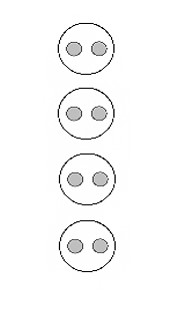
\includegraphics[height=0.95\textwidth]{invlf_fig5a.jpg}
	\caption{Lijn lay-out}
\end{subfigure}%
\begin{subfigure}{0.3\textwidth}
	\centering
	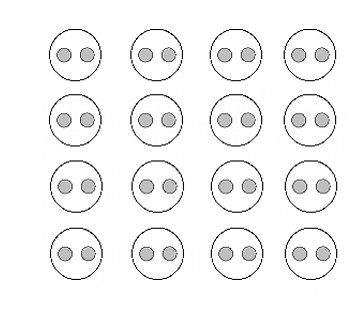
\includegraphics[height=0.95\textwidth]{invlf_fig5b.jpg}
	\caption{Matrix lay-out}
\end{subfigure}
\label{fig:invlf_5}
\centering
\caption{Mogelijke lay-outs van een boorgatenergieopslagveld.}
\end{figure}

\begin{figure}[hbtp] 
\begin{subfigure}{0.75\textwidth}
	\centering
	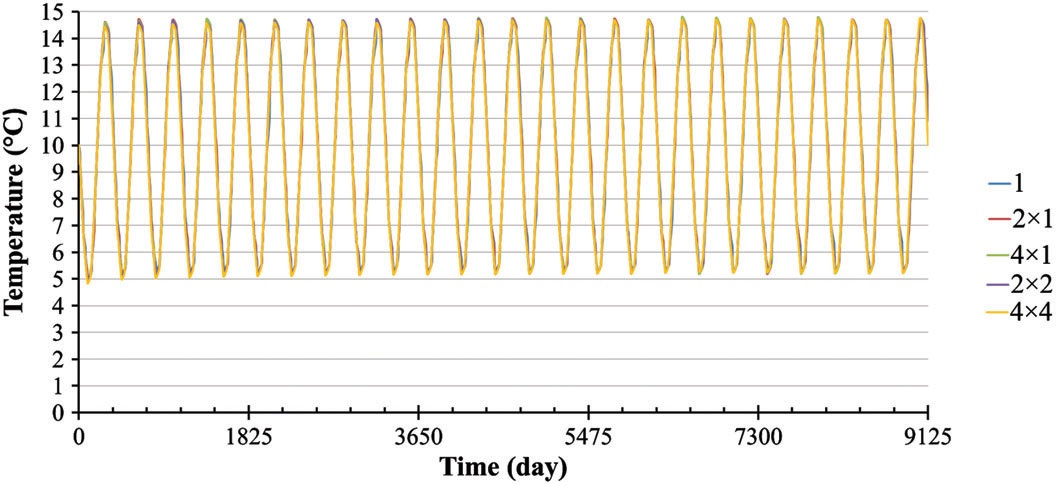
\includegraphics[width=0.75\textwidth]{invlf_fig6a.jpg}
	\caption{Gebalanceerde vraag met grondwaterstroming.}
\end{subfigure}
\begin{subfigure}{0.75\textwidth}
	\centering
	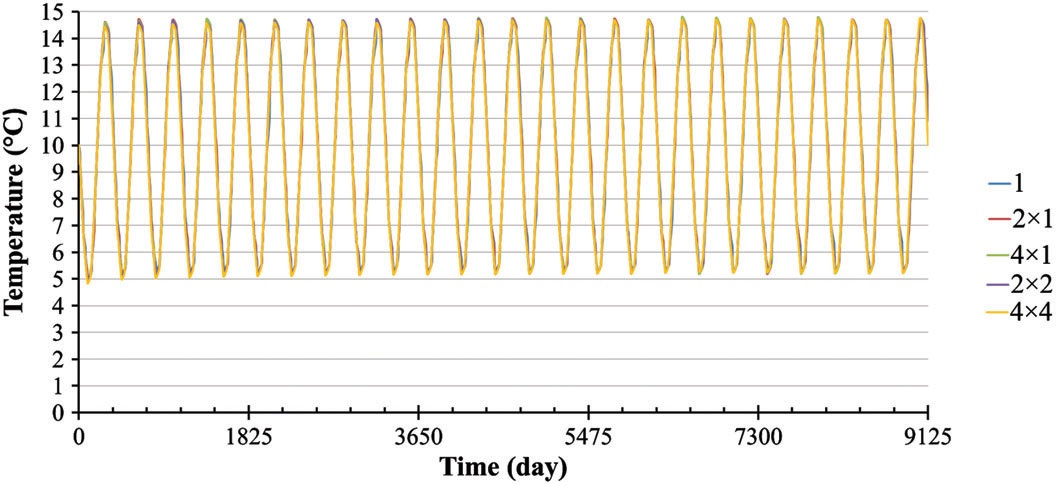
\includegraphics[width=0.75\textwidth]{invlf_fig6a.jpg}
	\caption{Ongebalanceerde vraag met grondwaterstroming.}
\end{subfigure}
\label{fig:invlf_6}
\centering
\caption{De grondtemperatuur doorheen de tijd.}
\end{figure}

\begin{figure}[hbtp] 
\begin{subfigure}{0.4\textwidth}
	\centering
	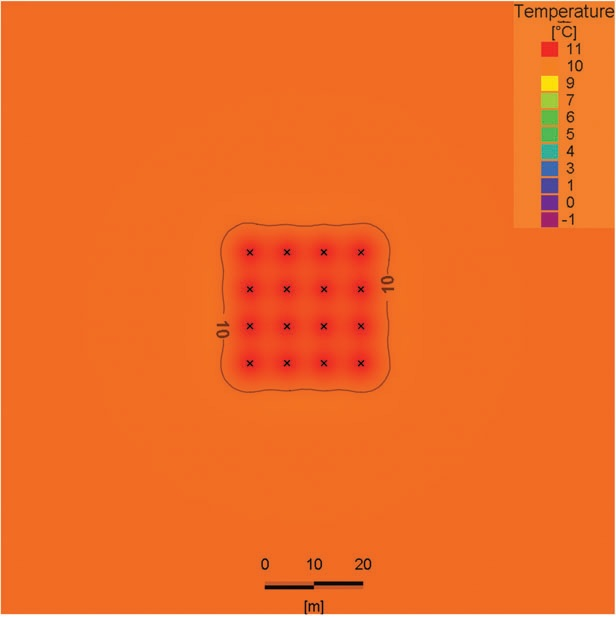
\includegraphics[width=0.95\textwidth]{invlf_fig7a.jpg}
	\caption[width=0.95\textwidth]{Gebalanceerde vraag zonder grondwaterstroming.}
\end{subfigure}%
\begin{subfigure}{0.4\textwidth}
	\centering
	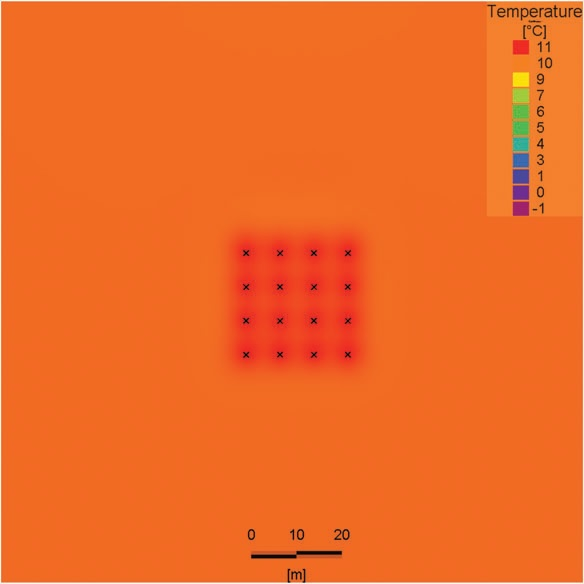
\includegraphics[width=0.95\textwidth]{invlf_fig7b.jpg}
	\caption[width=0.95\textwidth]{Gebalanceerde vraag met grondwaterstroming.}
\end{subfigure}
\begin{subfigure}{0.4\textwidth}
	\centering
	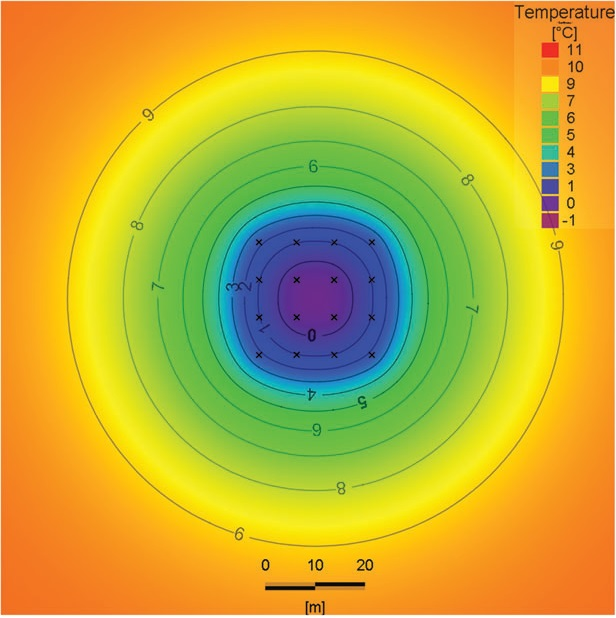
\includegraphics[width=0.95\textwidth]{invlf_fig7c.jpg}
	\caption[width=0.95\textwidth]{Ongebalanceerde vraag zonder grondwaterstroming.}
\end{subfigure}%
\begin{subfigure}{0.4\textwidth}
	\centering
	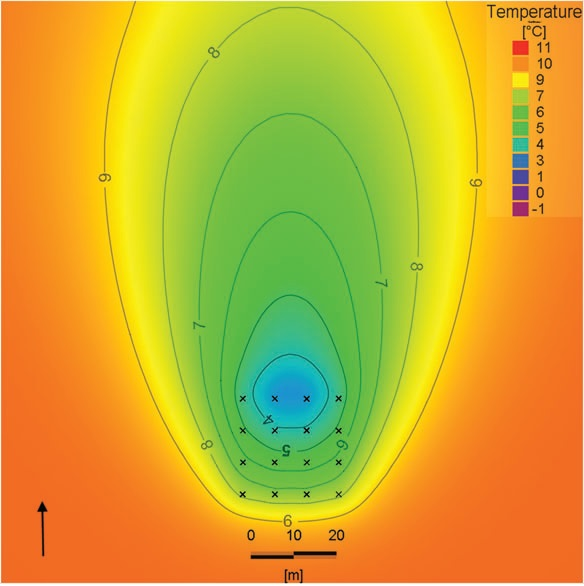
\includegraphics[width=0.95\textwidth]{invlf_fig7d.jpg}
	\caption[width=0.95\textwidth]{Ongebalanceerde vraag met grondwaterstroming.}
\end{subfigure}%
\label{fig:invlf_7}
\centering
\caption{De temperatuursverdeling van een boorgatenergieopslagveld met matrix lay-out in verschillende situaties van vraag en grondwaterstroming.}
\end{figure}

\begin{figure}[hbtp] 
\begin{subfigure}{0.4\textwidth}
	\centering
	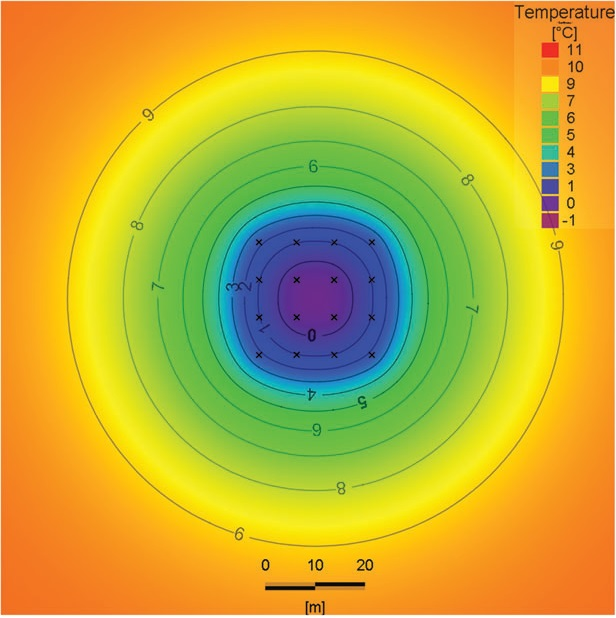
\includegraphics[width=0.95\textwidth]{invlf_fig8a.jpg}
	\caption{Matrix lay-out.}
\end{subfigure}%
\begin{subfigure}{0.4\textwidth}
	\centering
	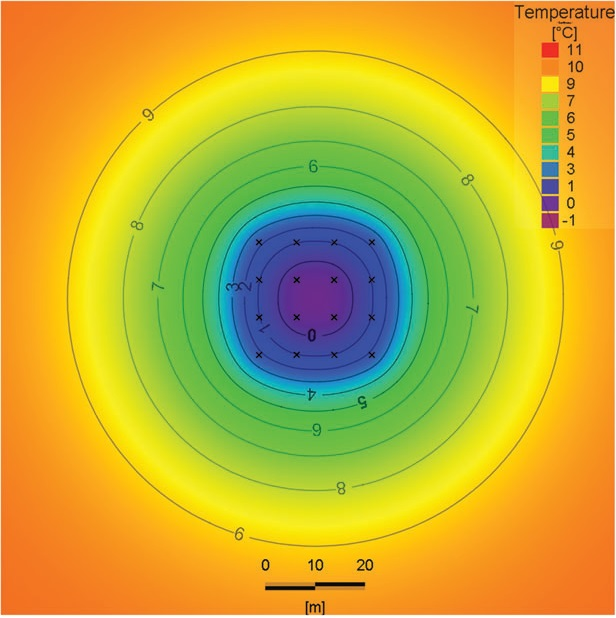
\includegraphics[width=0.95\textwidth]{invlf_fig8a.jpg}
	\caption{Lijn lay-out.}
\end{subfigure}%
\label{fig:invlf_8}
\centering
\caption{De temperatuursverdeling van een boorgatenergieopslagveld bij verschillende lay-outs met een ongebalanceerde warmtevraag en zonder grondwaterstroming.}
\end{figure}


\subsection*{Bodemsaturatie}
De graad van bodemsaturatie $S$ geeft de waterinhoud van de bodem weer. De waarde van $S$ ligt tussen 0 en de porositeit $\varphi$. 
\begin{equation}\label{invlf_eq3}
S=\dfrac{V_{water}}{V_{water}+v_{lucht}+V_{materiaal}}
\end{equation}
De bodemsaturatie is afhankelijk van de locatie in het boorgatenergieopslagveld. Bij een stijgende graad van saturatie, stijgt de thermische conductiviteit $k$ alsook de thermische diffusiviteit $\alpha$. Aangezien de bodemsaturatie ook verandert in de tijd, zijn de thermische conductiviteit en thermische diffusiviteit ook tijdsafhankelijk \cite{R2}.

\textcolor{red}{Figuur invoegen}

% Na de bijlagen plaatst men nog de bibliografie.
% Je kan de  standaard "abbrv" bibliografiestijl vervangen door een andere.
\bibliographystyle{abbrv}
\bibliography{referenties}


\end{document}

\chapter{Een volgend hoofdstuk}
\label{hoofdstuk:2}
Een hoofdstuk behandelt een samenhangend geheel dat min of meer op zichzelf
staat. Het is dan ook logisch dat het begint met een inleiding, namelijk
het gedeelte van de tekst dat je nu aan het lezen bent.

\section{Eerste onderwerp in dit hoofdstuk}
De inleidende informatie van dit onderwerp.

\subsection{Een item}
Een tekst staat nooit alleen. Dit wil zeggen dat er zeker ook referenties
nodig zijn. Dit kan zowel naar on-line documenten\cite{wiki} als naar
boeken\cite{pratchett06:_good_omens}.

\section{Figuren}
Figuren worden gebruikt om illustraties toe te voegen. Dit is dan ook de
manier om beeldmateriaal toe te voegen zoals getoond wordt in
figuur~\ref{fig:logo}.

\begin{figure}
  \centering
  \includegraphics{logokul}
  \caption{Het KU~Leuven logo.}
  \label{fig:logo}
\end{figure}

\section{Tabellen}
Tabellen kunnen gebruikt worden om informatie op een overzichtelijke te
groeperen. Een tabel is echter geen rekenblad! Vergelijk maar eens
tabel~\ref{tab:verkeerd} en tabel~\ref{tab:juist}. Welke tabel vind jij het
duidelijkst?

\begin{table}
  \centering
  \begin{tabular}{||l|lr||} \hline
    gnats     & gram      & \$13.65 \\ \cline{2-3}
              & each      & .01 \\ \hline
    gnu       & stuffed   & 92.50 \\ \cline{1-1} \cline{3-3}
    emu       &           & 33.33 \\ \hline
    armadillo & frozen    & 8.99 \\ \hline
  \end{tabular}
  \caption{Een tabel zoals het niet moet.}
  \label{tab:verkeerd}
\end{table}

\begin{table}
  \centering
  \begin{tabular}{@{}llr@{}} \toprule
    \multicolumn{2}{c}{Item} \\ \cmidrule(r){1-2}
    Animal    & Description & Price (\$)\\ \midrule
    Gnat      & per gram    & 13.65 \\
              & each        & 0.01 \\
    Gnu       & stuffed     & 92.50 \\
    Emu       & stuffed     & 33.33 \\
    Armadillo & frozen      & 8.99 \\ \bottomrule
  \end{tabular}
  \caption{Een tabel zoals het beter is.}
  \label{tab:juist}
\end{table}

\section{Lorem ipsum}
Tenslotte gaan we hier nog wat tekst voorzien zodat er minstens een
bijkomende bladzijde aangemaakt wordt. Dat geeft de gelegenheid om eens te
zien hoe de koptekst en de voettekst zich gedragen.

\subsection{Lorem ipsum dolor sit amet, consectetur adipiscing elit}
Sed nec tortor id felis tristique sodales. Nulla nec massa eu dui fermentum
tincidunt. Integer ullamcorper ante eget eros posuere faucibus. Nam id
ligula ut augue pulvinar vulputate id at purus. Aenean condimentum tortor
eu mi placerat eget eleifend massa mollis. Nam est mi, sagittis quis
euismod eget, sagittis in nibh. Proin elit turpis, aliquam et imperdiet
sed, volutpat eu turpis.

Pellentesque vel enim tellus, vitae egestas turpis. Praesent malesuada elit
non nisi sollicitudin non blandit lacus tincidunt. Morbi blandit urna at
lectus ornare laoreet. Suspendisse turpis diam, lobortis dictum luctus
quis, commodo at lorem. Integer lacinia convallis ultricies. Sed quis augue
neque, eu malesuada arcu. Nullam vehicula, purus vitae sagittis pulvinar,
erat eros semper massa, eu egestas nibh erat quis magna. Cras pellentesque,
nisl eu dapibus volutpat, urna augue ornare quam, quis egestas lectus nulla
a lectus.

Vivamus dictum libero in massa cursus sed vulputate eros imperdiet. Donec
lacinia, libero ac lobortis egestas, nibh dui ornare arcu, luctus porttitor
velit massa sit amet quam. Maecenas scelerisque laoreet diam, vitae congue
quam adipiscing vitae. Aliquam cursus nisl a leo convallis eleifend
fermentum massa porta. Nunc libero quam, dapibus dapibus molestie sit amet,
faucibus vel nunc.

\subsection{Praesent auctor venenatis posuere}
Sed tellus augue, molestie in pulvinar lacinia, dapibus non ipsum. Fusce
vitae mi vitae enim ullamcorper hendrerit eu malesuada est. Proin iaculis
ante sed nibh tincidunt vel interdum libero posuere. Vivamus accumsan metus
quis felis congue suscipit dapibus enim mattis. Fusce mattis tortor eget
ipsum interdum sagittis auctor id metus.

Integer diam lacus, pharetra sit amet tempor et, tristique non lorem.
Aenean auctor, nisi eu interdum fermentum, lectus massa adipiscing elit,
sed facilisis orci odio a lectus. Proin mi nibh, tempus quis porta a,
viverra quis enim. In sollicitudin egestas libero, quis viverra velit
molestie eget. Nulla rhoncus, dolor a mollis vestibulum, lacus elit semper
nisi, nec sollicitudin sem urna eu magna. Nunc sed est urna, euismod congue
mi.

\subsection{Cras vulputate ultricies venenatis}
Vivamus eros urna, sodales accumsan semper vel, lobortis sit amet mauris.
Etiam condimentum eleifend lorem, ullamcorper ornare lectus aliquet vitae.
Praesent massa enim, interdum sit amet semper et, venenatis ut elit.
Quisque faucibus, quam ac lacinia imperdiet, nulla neque elementum purus,
tempus rutrum justo massa porta sapien. Vestibulum ante ipsum primis in
faucibus orci luctus et ultrices posuere cubilia Curae; Sed ultrices
interdum mi, et rhoncus sapien rutrum sed.

Duis elit orci, molestie quis sollicitudin sed, convallis non ante.
Maecenas tincidunt condimentum justo, et ultricies leo tristique vitae.
Vestibulum quis quam non lectus dapibus eleifend a vitae nibh. Nam nibh
justo, pharetra quis iaculis consequat, elementum quis justo. Etiam mollis
lacinia lacus, nec sollicitudin urna lobortis ac. Nulla facilisi.

Proin placerat risus eleifend erat ultricies placerat. Etiam rutrum magna
nec turpis euismod consectetur. Phasellus tortor odio, lacinia imperdiet
condimentum sed, faucibus commodo erat. Phasellus sed felis id ante
placerat ultrices. Aenean tempor justo in tortor volutpat eu auctor dolor
mollis. Aenean sit amet risus urna. Morbi viverra vehicula cursus.

\subsection{Donec nibh ante, consectetur et posuere id, tempus nec arcu}
Curabitur a tellus aliquet ipsum pellentesque scelerisque. Etiam congue,
risus et volutpat rutrum, est purus dapibus leo, non cursus metus felis
eget ligula. Vivamus facilisis tristique turpis, ut pretium lectus luctus
eleifend. Fusce magna sapien, ullamcorper vitae fringilla id, euismod quis
ante.

Phasellus volutpat, nunc et pharetra semper, sem justo adipiscing mauris,
id blandit magna quam et orci. Vestibulum a erat purus, ut molestie ante.
Vestibulum ante ipsum primis in faucibus orci luctus et ultrices posuere
cubilia Curae; Proin turpis diam, consequat ut ullamcorper ut, consequat eu
orci. Sed metus risus, fringilla nec interdum vel, interdum eu nunc.
Suspendisse vel sapien orci.

\subsection{Morbi et mauris tempus purus ornare vehicula}
Mauris sit amet diam quam, eget luctus purus. Sed faucibus, risus semper
eleifend iaculis, mi turpis bibendum nisl, quis cursus nibh nisl sit amet
ipsum. Vestibulum tempor urna vitae mi auctor malesuada eget non ligula.
Nullam convallis, diam vel ultrices auctor, eros eros egestas elit, sed
accumsan arcu tortor eget leo. Vestibulum orci purus, porttitor in pharetra
eget, tincidunt eget nisl. Nullam sit amet nulla dui, facilisis vestibulum
dui.

Donec faucibus facilisis mauris ac cursus. Duis rhoncus quam sed nisi
laoreet eu scelerisque massa tincidunt. Vivamus sit amet libero nec arcu
imperdiet tempor quis non libero. Sed consequat dignissim justo. Phasellus
ullamcorper, velit quis posuere vulputate, felis erat tincidunt mauris, at
vestibulum justo lectus et turpis. Maecenas lacinia convallis euismod.
Quisque egestas fermentum sapien eu dictum. Sed nec lacus in purus dictum
consequat quis vel nisl. Fusce non urna sem. Curabitur eu diam vitae elit
accumsan blandit. Nullam fermentum nunc et leo dictum laoreet. Donec semper
varius velit vel fringilla. Vivamus eu orci nunc.

\section{Besluit van dit hoofdstuk}
Als je in dit hoofdstuk tot belangrijke resultaten of besluiten gekomen
bent, dan is het ook logisch om het hoofdstuk af te ronden met een
overzicht ervan. Voor hoofdstukken zoals de inleiding en het
literatuuroverzicht is dit niet strikt nodig.

%%% Local Variables: 
%%% mode: latex
%%% TeX-master: "masterproef"
%%% End: 

% ... en zo verder tot
\chapter{Het laatste hoofdstuk}
\label{hoofdstuk:n}
Een hoofdstuk behandelt een samenhangend geheel dat min of meer op zichzelf
staat. Het is dan ook logisch dat het begint met een inleiding, namelijk
het gedeelte van de tekst dat je nu aan het lezen bent.

\section{Eerste onderwerp in dit hoofdstuk}
De inleidende informatie van dit onderwerp.

\subsection{Een item}
De bijbehorende tekst. Denk eraan om de paragrafen lang genoeg te maken en
de zinnen niet te lang.

Een paragraaf omvat een gedachtengang en bevat dus steeds een paar zinnen.
Een paragraaf die maar \'e\'en lijn lang is, is dus uit den boze.

\section{Tweede onderwerp in dit hoofdstuk}
Er zijn in een hoofdstuk verschillende onderwerpen. We zullen nu
veronderstellen dat dit het laatste onderwerp is.

\section{Besluit van dit hoofdstuk}
Als je in dit hoofdstuk tot belangrijke resultaten of besluiten gekomen
bent, dan is het ook logisch om het hoofdstuk af te ronden met een
overzicht ervan. Voor hoofdstukken zoals de inleiding en het
literatuuroverzicht is dit niet strikt nodig.

%%% Local Variables: 
%%% mode: latex
%%% TeX-master: "masterproef"
%%% End: 

\chapter{Besluit}
\label{besluit}
De masterproeftekst wordt afgesloten met een hoofdstuk waarin alle
besluiten nog eens samengevat worden. Dit is ook de plaats voor suggesties
naar het verder gebruik van de resultaten, zowel industri"ele toepassingen
als verder onderzoek.

\lipsum[1-7]

%%% Local Variables: 
%%% mode: latex
%%% TeX-master: "masterproef"
%%% End: 


% Indien er bijlagen zijn:
\appendixpage*          % indien gewenst
\appendix
\chapter{De eerste bijlage}
\label{app:A}
In de bijlagen vindt men de data terug die nuttig kunnen zijn voor de
lezer, maar die niet essentieel zijn om het betoog in de normale tekst te
kunnen volgen. Voorbeelden hiervan zijn bronbestanden,
configuratie-informatie, langdradige wiskundige afleidingen, enz.

In een bijlage kunnen natuurlijk ook verdere onderverdelingen voorkomen,
evenals figuren en referenties\cite{h2g2}.

\section{Meer lorem}
\lipsum[50]

\subsection{Lorem 15--17}
\lipsum[15-17]

\subsection{Lorem 18--19}
\lipsum[18-19]

\section{Lorem 51}
\lipsum[51]

%%% Local Variables: 
%%% mode: latex
%%% TeX-master: "masterproef"
%%% End: 

% ... en zo verder tot
\chapter{De laatste bijlage}
\label{app:n}
In de bijlagen vindt men de data terug die nuttig kunnen zijn voor de
lezer, maar die niet essentieel zijn om het betoog in de normale tekst te
kunnen volgen. Voorbeelden hiervan zijn bronbestanden,
configuratie-informatie, langdradige wiskundige afleidingen, enz.

\section{Lorem 20-24}
\lipsum[20-24]

\section{Lorem 25-27}
\lipsum[25-27]

%%% Local Variables: 
%%% mode: latex
%%% TeX-master: "masterproef"
%%% End: 


\backmatter
% Na de bijlagen plaatst men nog de bibliografie.
% Je kan de  standaard "abbrv" bibliografiestijl vervangen door een andere.
\bibliographystyle{abbrv}
\bibliography{referenties}

\end{document}

%%% Local Variables: 
%%% mode: latex
%%% TeX-master: t
%%% End: 
